\documentclass[]{scrartcl}
\usepackage{graphicx}
\usepackage{color}
\usepackage[ngerman]{babel}
\usepackage{hyperref}
\usepackage{fullpage}
\usepackage{calc} 
\usepackage{enumitem}
\usepackage{titlesec}
\newcommand{\todo}[1]{\textcolor{red}{TODO: #1}\PackageWarning{TODO:}{#1!}}
\begin{document}

\title{
	\includegraphics*[width=0.75\textwidth]{images/hu_logo.png}\\
	\vspace{24pt}
	Wittgenstein:\\Tractatus Logico-Philosophicus}
\subtitle{Proseminar WS 16/17\\
          Dr. Jasper Liptow\\
          Philosophisches Institut I \\ 
          Humboldt Universit"at zu Berlin}
\author{Lennard Wolf\\
        \href{mailto:lennard.wolf@student.hu-berlin.de}{lennard.wolf@student.hu-berlin.de}}
\maketitle
\begin{abstract}

In seinem Tractatus logico-philosophicus (1921) pr"asentiert Ludwig Wittgenstein in atemberaubend dichter Form "Uberlegungen zum Wesen der Sprache, der Logik, der Welt und nicht zuletzt der Philosophie selbst. Seine Charakterisierung des Tractatus im Vorwort lautet kurz: \emph{Das Buch behandelt die philosophischen Probleme und zeigt – wie ich glaube – dass die Fragestellung dieser Probleme auf dem Missverst"andnis der Logik unserer Sprache beruht. Man k"onnte den ganzen Sinn des Buches etwa in die Worte fassen: Was sich "uberhaupt sagen l"asst, l"asst sich klar sagen; und wovon man nicht reden kann, dar"uber muss man schweigen.} Diese Zeilen deuten bereits an, warum der Tractatus einen der entscheidenden Schritte auf dem Weg zu einer inhaltlichen und methodischen Orientierung der Philosophie an der Sprache darstellt, wie sie die Philosophie des 20. Jahrhunderts gepr"agt hat (linguistic turn). 
Im Seminar wollen wir zum einen versuchen, den Gedankengang des Tractatus anhand einer genauen Lekt"ure zu rekonstruieren, und gucken, welche der Schmuckst"ucke aus dieser \emph{jewel box of insights} (wie der amerikanische Philosoph Wilfrid Sellars den Tractatus einmal nennt) bis heute ihren Glanz bewahrt haben.


\end{abstract}
\newpage

\tableofcontents
\newpage


\section{Einf"uhrende Sitzung\\(31.10.16)}

\textbf{Zu lesen:} 

\emph{Wittgenstein's Tractatus logico-philosophicus: A Reader's Guide} von Roger White

Selbst gefunden: 
\emph{Sprache und Wirklichkeit in Wittgensteins Tractatus} von Rolf-Albert Dietrich | \url{https://books.google.no/books?id=mwe1KLQM3bYC}

\subsection{Einfl"usse}

In einer Liste seiner Einfl"usse war Schopenhauer der einzige Philosoph, den Wittgenstein auff"uhrte. Am wichtigsten waren jedoch Frege und Russell.

\begin{description}[leftmargin=!,labelwidth=\widthof{\bfseries 2}]
  \item[Frege] War Vertreter des \emph{Logizismus} und verfolte daher das Ziel zu zeigen, dass die Axiome der Arithmetik sich aus den Axiomen der Logik herleiten lassen. Er entwickelte in seiner \emph{Begriffsschrift} die Pr"adikatenlogik erster Stufe. In seinem Buch \emph{Die Grundlagen der Arithmetik}, welches die Frage `\emph{Was sind Zahlen?}' thematisiert, stellt er das \emph{Kontextprinzip} vor, demnach Begriffe nur im Zusammenhang eines Satzes etwas bedeuten. So erh"alt etwa der Begriff `Stein' erst eine Bedeutung, wenn er im Elementarsatz `$x$ ist ein Stein' auftritt. In \emph{Grundgesetze der Arithmetik} wollte er den Logizismus voll implementieren, doch die Einf"uhrung der Mengentheorie als Axiom der Logik produzierte ein Paradox, welches von Russell erkannt wurde (z.B. Die Menge er Mengen, die sich nicht selbst inkludieren).
  \item[Russell] 
\end{description}

\subsection{Vorwort}

\emph{Das Buch will also dem Denken eine Grenze ziehen, oder vielmehr – nicht dem Denken, sondern dem Ausdruck der Gedanken: Denn um dem Denken eine Grenze zu ziehen, m"ußten wir beide Seiten dieser Grenze denken k"onnen.} Wittgensteins Hauptanliegen ist es, die Philosophie von Unsinn und Verwirrung zu bereinigen, denn \emph{[d]ie meisten S"atze und Fragen, welche "uber philosophische Dinge geschrieben worden sind, sind nicht falsch, sondern unsinnig. Wir k"onnen daher Fragen dieser Art "uberhaupt nicht beantworten, sondern nur ihre Unsinnigkeit feststellen. Die meisten Fragen und S"atze der Philosophen beruhen darauf, dass wir unsere Sprachlogik nicht verstehen.} (4.003)

Die Grenzziehung in der Sprache wird die Grenzziehung zwischen \emph{sinnvollen}, \emph{sinnlosen} und \emph{unsinnigen} S"atzen sein.

\subsection{Die S"atze der ersten Gliederungsebene}
\begin{description}[leftmargin=!,labelwidth=\widthof{\bfseries 12}]
  \item[1] Die Welt ist alles, was der Fall ist.
  \item[2] Was der Fall ist, die Tatsache, ist das Bestehen von Sachverhalten.
  \item[3] Das logische Bild der Tatsachen ist der Gedanke.
  \item[4] Der Gedanke ist der sinnvolle Satz.
  \item[5] Der Satz ist eine Wahrheitsfunktion der Elementars"atze.\\
(Der Elementarsatz ist eine Wahrheitsfunktion seiner selbst.)
  \item[6] Die allgemeine Form der Wahrheitsfunktion ist: $[~\bar{p},~\bar{\xi},~N(\bar{\xi})~]$.\\
Dies ist die allgemeine Form des Satzes.
  \item[7] Wovon man nicht sprechen kann, dar"uber muss man schweigen.
\end{description}

\section{Gegenstand, Sachverhalt, Tatsache: 1 bis 2.063\\(07.11.16)}
\subsection{Lekt"urenotizen}
\textbf{Gedanken zum Text}

Wittgenstein scheint in diesem Abschnitt zum einen eine terminologische Grundlage f"ur den Rest des Textes legen zu wollen, zum anderen werden aber auch schon gewissen ontologische Aussagen getroffen, zum Beispiel durch \emph{Die Welt ist die Gesamtheit der Tatsachen, nicht der Dinge.} (1.1). Ich stelle mir die nun folgende Struktur des Textes so vor, dass erst eine Ontologie entworfen wird und dann gezeigt wird, wie die Sprache (und damit das Denken?) mit der in dieser Ontologie entworfenen `Welt' in Beziehung steht. 

\vspace{10pt}
\textbf{Neue Begriffe}

\begin{description}[leftmargin=!,labelwidth=\widthof{\bfseries Konfiguration}]
  \item[Welt] \emph{Alles} was der Fall ist. Die Gesamtheit der Tatsachen, d.h. der bestehenden Sachverhalte.
  \item[Tatsache] Das Bestehen von Sachverhalten. (\emph{Was der Fall ist})
  \item[Gegenstand] Ein einfaches Ding das nicht teilbar ist. $\rightarrow$ Auch \emph{Ding} genannt. | Um ihn zu \emph{kennen}, muss ich alle seine internen Eigenschaften kennen, d.h. auch s"amtliche M"oglichkeiten seines Vorkommens in Sachverhalten (diese liegen in seiner Natur). | Identit"at ist keine Relation zwischen Gegenst"anden.
  \item[Sachverhalt] Eine Verbindung von Gegenst"anden.
  \item[Sachlage] Ein Komplex aus Sachverhalten.
  \item[Struktur] \emph{Die Art und Weise, wie die Gegenst"ande im Sachverhalt zusammenh"angen, ist die Struktur des Sachverhaltes.} (2.032)
  \item[Form] \emph{Die Form} [des Gegenstands] \emph{ist die M"oglichkeit der Struktur.} (2.033), oder auch auch \emph{die M"oglichkeit seines Vorkommens in Sachverhalten}. (2.0141)
  \item[Substanz] Die Substanz der Welt ist gebildet durch die (unteilbaren) Gegenst"ande. Sie besteht unabh"angig von dem, was der Fall ist. (s. 2.024)
  \item[Konfiguration] Die Konfiguration der Gegenst"ande bildet den Sachverhalt. Die ist das Wechselnde, Unbest"andige (im Gegensatz zu den Gegenst"anden).
  \item[Wirklichkeit] \emph{Das Bestehen und Nichtbestehen von Sachverhalten ist die Wirklichkeit.} (2.06) | \emph{Sind alle Gegenst"ande gegeben, so sind damit auch alle m"oglichen Sachverhalte gegeben.} (2.0124) | \emph{Die gesamte Wirklichkeit ist die Welt.} (2.063) {\color{red}(Was w"are halbe Wirklichkeit?)}
\end{description}

\textbf{Fragen}

\begin{itemize}
  \item \emph{Eines kann der Fall sein oder nicht der Fall sein und alles "ubrige bleibt gleich} (1.21) | Soll das hei\ss en, dass Tatsachen voneinander unabh"angig sind? $\rightarrow$ steht in (2.061), aber was hei\ss t das? Wie spielt Zeit/Kausalit"at da rein?
  \item \emph{Die Substanz der Welt besteht unabh"angig von dem, was der Fall ist.} (2.024) Hei\ss t das, dass ohne eine Konfiguration die Substanz ein formloser `Blob' ist?
  \item Unterschied Welt und Wirklichkeit? Welt hat Substanz, Wirklichkeit ist nur eine `Wahrheitstafel'? 
  \item \emph{Wie} atomar sind denn die Gegenst"ande? Ist ein Tisch ein Gegenstand?
\end{itemize}


\section{Gegenstand, Sachverhalt, Tatsache: 1 bis 2.063\\(07.11.16)}

\section{Tatsache und Bild: 2.1 bis 3.01\\(14.11.16)}

\subsection{Lekt"urenotizen}
\textbf{Gedanken zum Text}

Wittgenstein scheint...

\vspace{10pt}
\textbf{Neue Begriffe}

\begin{description}[leftmargin=!,labelwidth=\widthof{\bfseries Sachverhalt}]
  \item[Bild] ...
  \item[Tatsache] 
\end{description}

\textbf{Fragen}

\begin{itemize}
  \item 
\end{itemize}

\section{Satz und Name: 3 bis 3.263\\(21.11.16)}


\subsection{Lekt"urenotizen}
\textbf{Gedanken zum Text}

Wittgenstein scheint...

\vspace{10pt}
\textbf{Neue Begriffe}

\begin{description}[leftmargin=!,labelwidth=\widthof{\bfseries Sachverhalt}]
  \item[Bild] ...
  \item[Tatsache] 
\end{description}

\textbf{Fragen}

\begin{itemize}
  \item 
\end{itemize}

\begin{center}
    \begin{tabular}{  l | l }
    \textbf{Wirklichkeit} & \textbf{Sprache}\\ \hline
    Gegenstand & Name \\ 
    Sachverhalt & Elementarsatz \\
    Sachlage & Satz \\
    \end{tabular}
\end{center}


\section{Primat des Satzsinns: 3.3 bis 3.5\\(28.11.16)}


\subsection{Lekt"urenotizen}
\textbf{Gedanken zum Text}

Wittgenstein scheint...

\vspace{10pt}
\textbf{Neue Begriffe}

\begin{description}[leftmargin=!,labelwidth=\widthof{\bfseries Sachverhalt}]
  \item[Bild] ...
  \item[Tatsache] 
\end{description}

\textbf{Fragen}

\begin{itemize}
  \item 
\end{itemize}



\newpage
\section{Anhang}

\begin{figure}[h]
	%\centering
	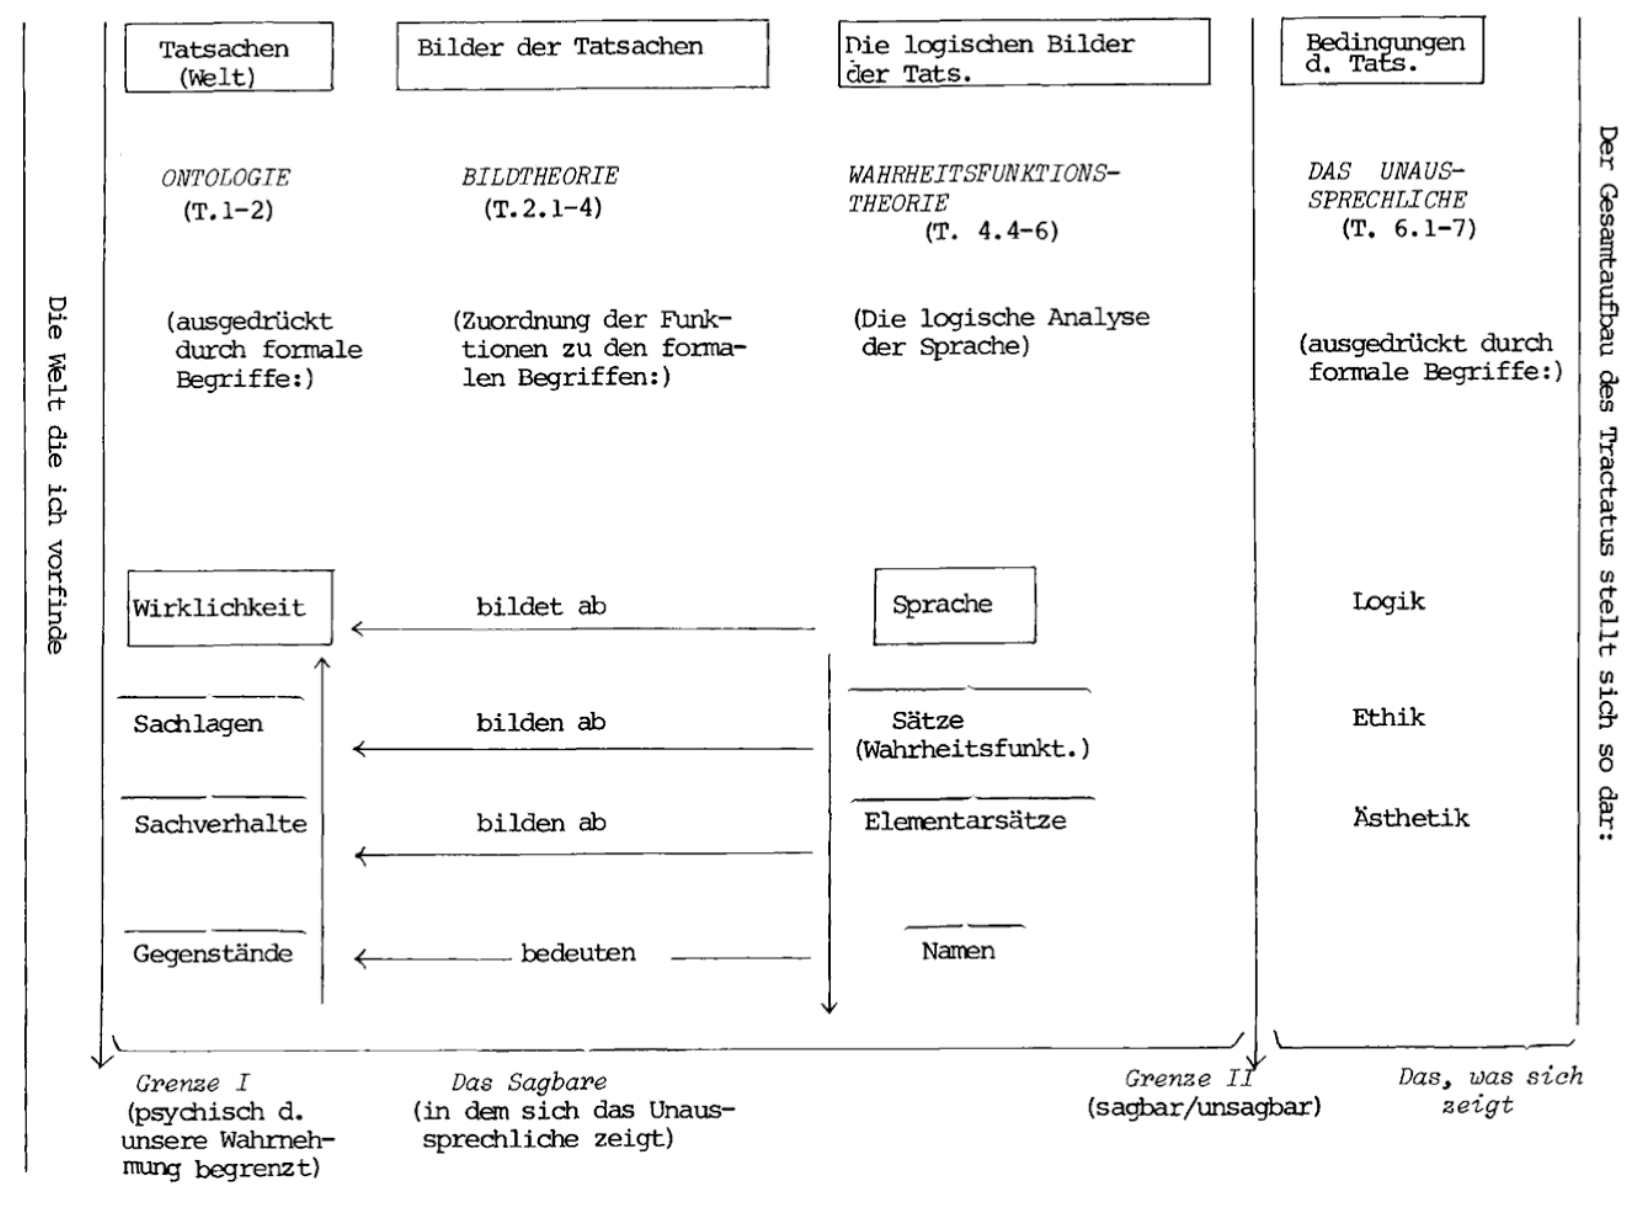
\includegraphics[width=1\textwidth]{images/tractatus-structur.png}
	\caption{Der Gesamtaufbau des Tractatus. Quelle: \emph{Sprache und Wirklichkeit in Wittgensteins Tractatus} von Rolf-Albert Dietrich}
	\label{fig:struct}
\end{figure}


\newpage
\section{"Uber den Dozenten}
Dr. Jasper Liptow absolvierte 1996 seinen Magister an der Universit"at Hamburg, promovierte in Gie\ss en mit einer Arbeit zum Thema \emph{Gebrauchstheorien der Bedeutung} bei Prof. Martin Seel und ist Privatdozent.


\begin{figure}[]
	\centering
	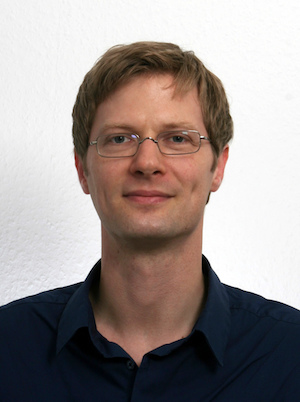
\includegraphics[width=0.32\textwidth]{images/liptow.jpg}
	\caption{Dr. Jasper Liptow. Quelle: \url{https://www.uni-frankfurt.de/45457854/liptow.jpg}}
	\label{fig:liptow}
\end{figure}

%\begin{figure}[h]
%	\centering
%	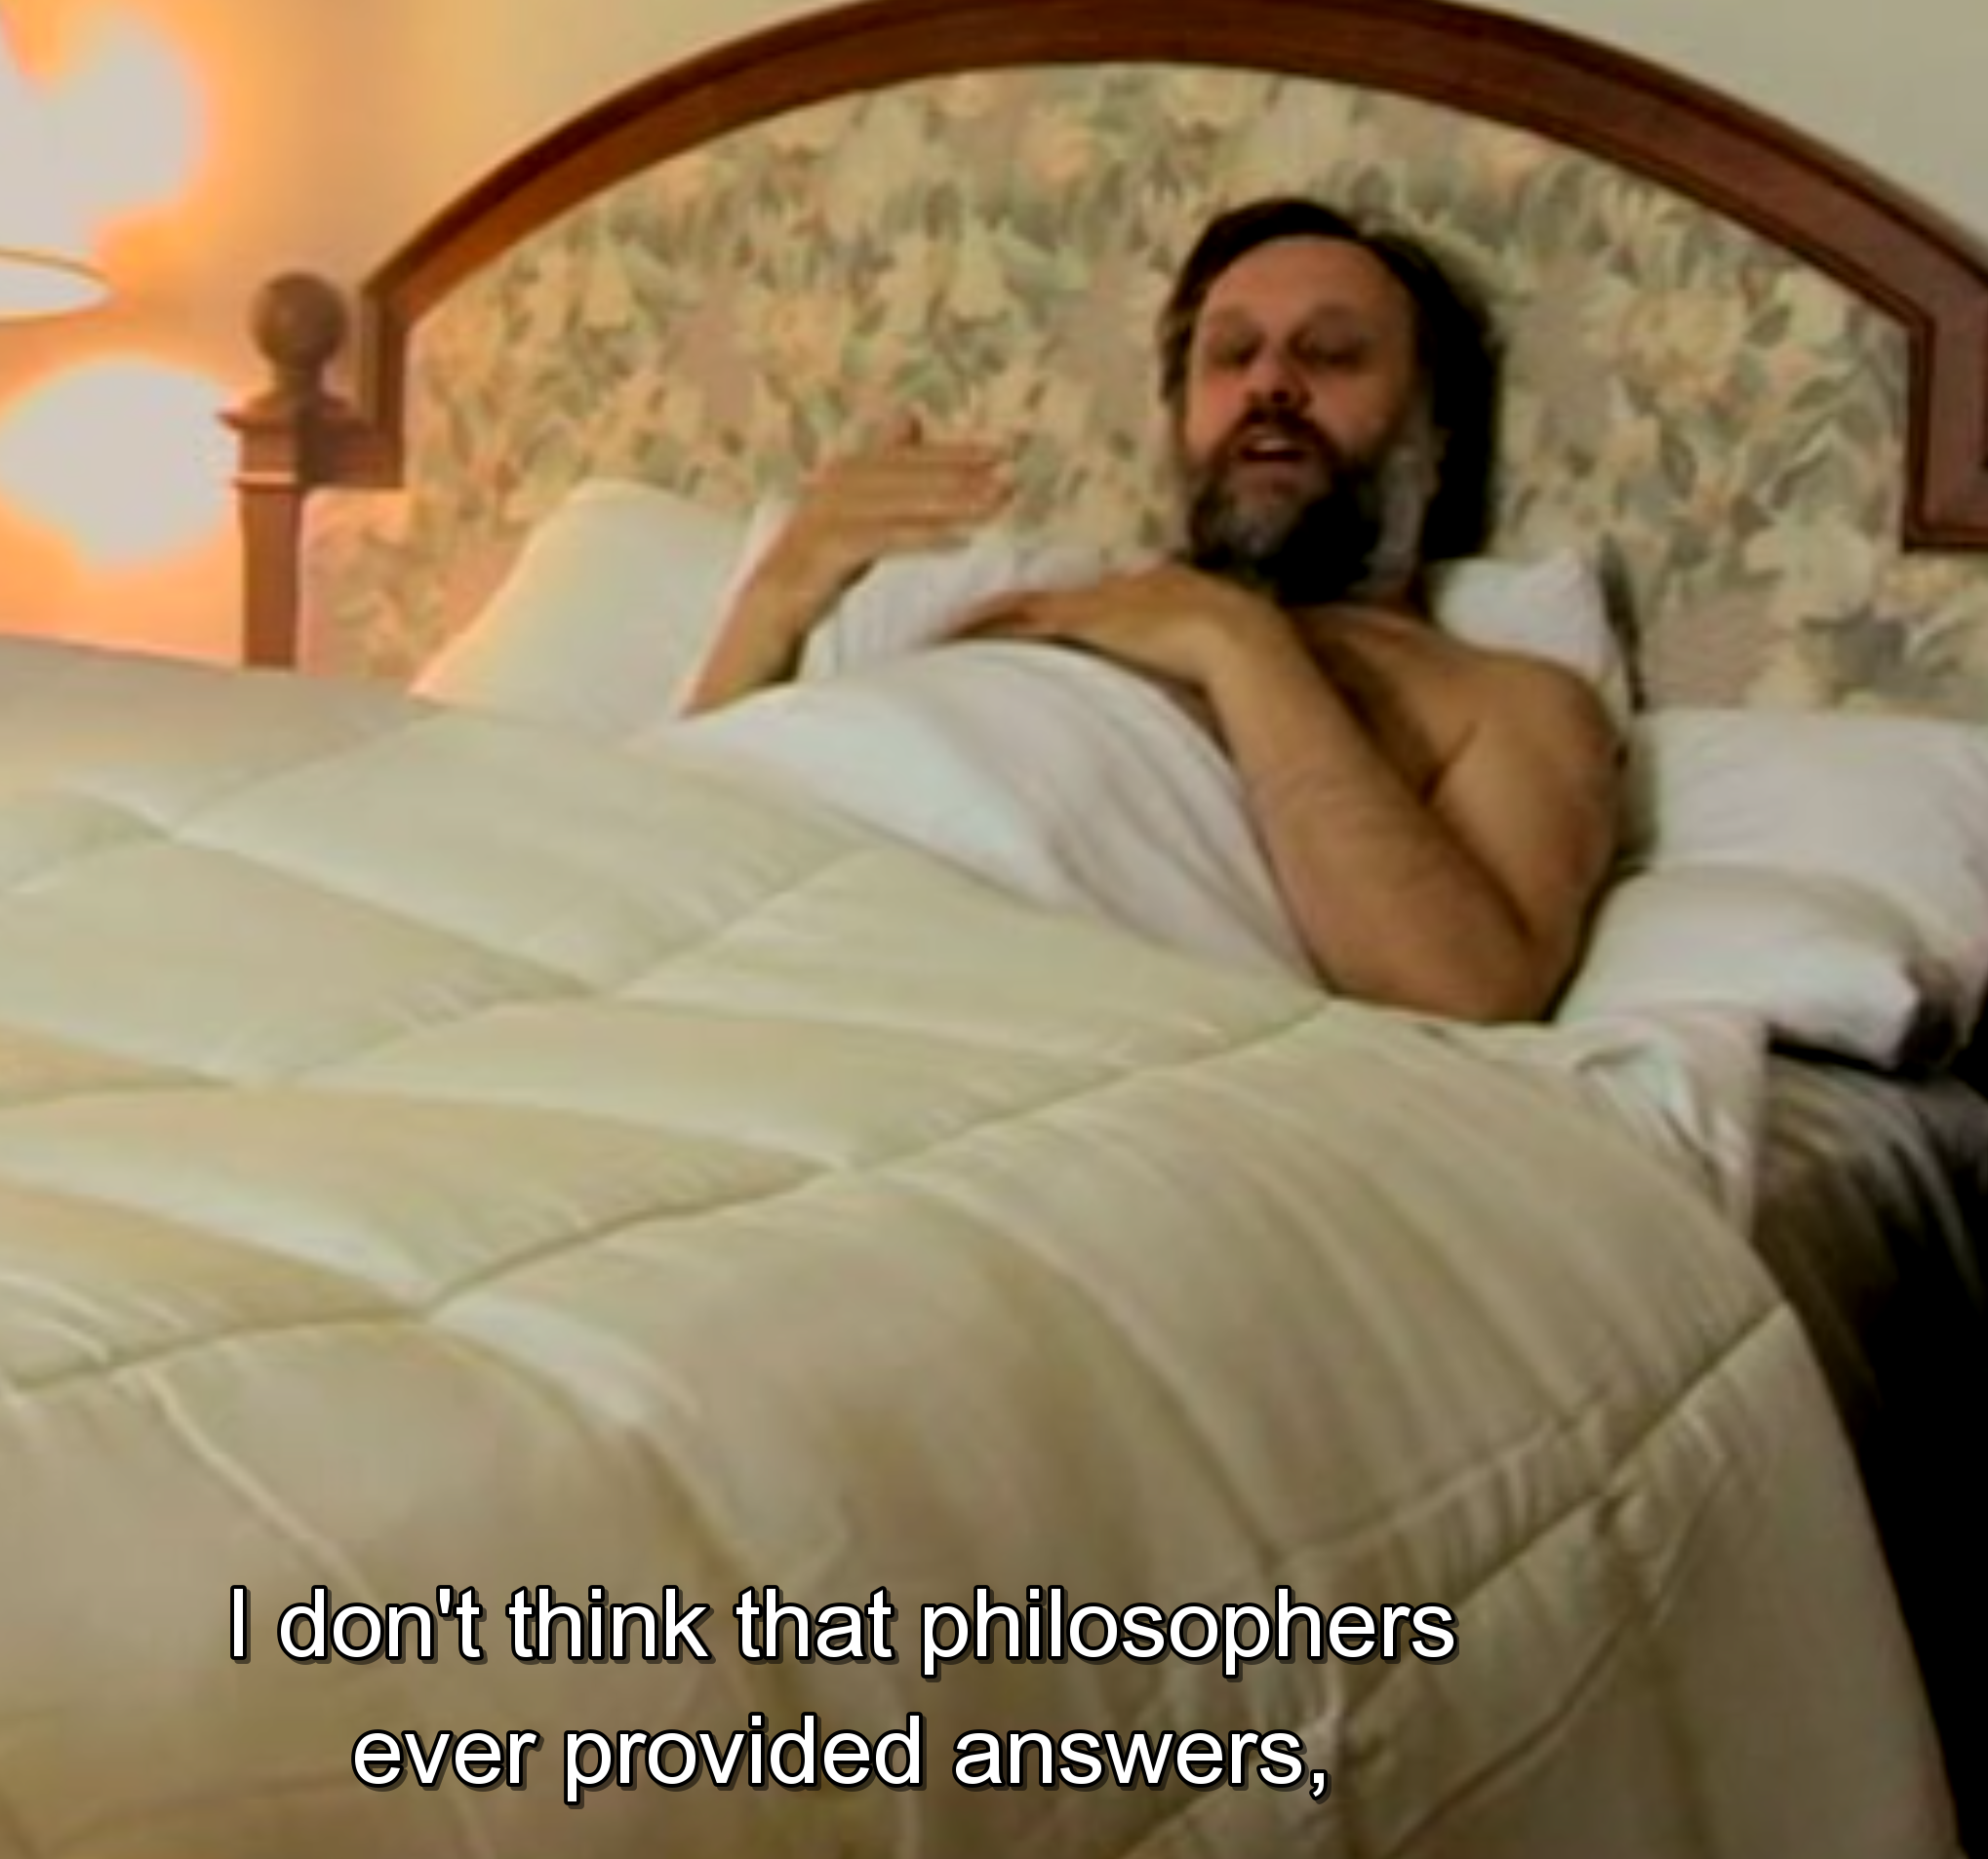
\includegraphics[width=0.5\textwidth]{images/template.png}
%	\caption{Template Bild}
%	\label{fig:template}
%\end{figure}

\end{document}
